% ============================================================
%  Derivation: 2D Cylindrical Coordinates (r, z)
%  Velocities: u (radial), w (axial)
%  Integration element: dr dz   (axisymmetric: no phi dependence)
% ============================================================

\section{2D Incompressible Flow in Cylindrical Coordinates $(r,z)$ --- Velocities $(u,w)$}
\label{sec:cyl_uw}

\emph{Note on notation:} this appendix derives the FVM discretisation, projection method,
and ghost-cell treatment in general form, illustrating $u$ and $w$ as cell-centred quantities
near each boundary for schematic clarity. The staggered grid actually implemented (Table~2 in
the main text) instead stores $u$ exactly \emph{at} the axis and wall faces and $w$ exactly
\emph{at} the inlet and outlet faces, so those boundary-normal components are set directly
(Dirichlet) rather than via a mirrored ghost cell; only the wall-tangential component and the
scalars ($p$, $\theta$) use the mirrored ghost-cell form shown here. The relaxation factor
$\zeta$ below is the same quantity as $\alpha_p$ in Section~\ref{sec:pressure-correction},
where this submission uses $\alpha_p = 0.7$.

\subsection{Governing Equations (Strong Form)}

For axisymmetric flow ($\partial/\partial\phi = 0$, $v_\phi = 0$) in cylindrical coordinates $(r,z)$:

\textbf{Continuity:}
\begin{equation}
    \frac{1}{r}\frac{\partial(ru)}{\partial r}+\frac{\partial w}{\partial z}
    = 0
    \label{eq:cyl_uw_cont}
\end{equation}

\textbf{Radial momentum ($r$-direction):}
\begin{equation}
    \frac{\partial u}{\partial t}
    + \frac{1}{r}\frac{\partial(ru^2)}{\partial r}
    + \frac{\partial(uw)}{\partial z}
    = -\frac{1}{\rho}\frac{\partial p}{\partial r}
    + \frac{1}{\rho r}\frac{\partial(r\tau_{rr})}{\partial r}
    + \frac{1}{\rho}\frac{\partial\tau_{rz}}{\partial z}
    \label{eq:cyl_uw_momr}
\end{equation}

\textbf{Axial momentum ($z$-direction):}
\begin{equation}
    \frac{\partial w}{\partial t}
    + \frac{1}{r}\frac{\partial(ruw)}{\partial r}
    + \frac{\partial(w^2)}{\partial z}
    = -\frac{1}{\rho}\frac{\partial p}{\partial z}
    + \frac{1}{\rho r}\frac{\partial(r\tau_{rz})}{\partial r}
    + \frac{1}{\rho}\frac{\partial\tau_{zz}}{\partial z}
    \label{eq:cyl_uw_momz}
\end{equation}

where for a Newtonian fluid with constant viscosity $\mu = \rho\nu$:
\begin{align}
    \tau_{rr} &= 2\mu\frac{\partial u}{\partial r}
    \\
    \tau_{zz} &= 2\mu\frac{\partial w}{\partial z}
    \\
    \tau_{rz} &= \mu\!\left(\frac{\partial u}{\partial z}+\frac{\partial w}{\partial r}\right)
\end{align}

% ----------------------------------------------------------
\subsection{Staggered Grid Layout}
% ----------------------------------------------------------

\begin{figure}[H]
\centering
\begin{tikzpicture}[scale=1.5, >=Latex]

% ---------------------------------------------------------------
% Front face (theta = theta_j): the (r,z) cross-section of one CV
% ---------------------------------------------------------------
\coordinate (A) at (0,0);       % r_i,     z_j
\coordinate (B) at (2.6,0);     % r_i,     z_{j+1}
\coordinate (C) at (2.6,1.8);   % r_{i+1}, z_{j+1}
\coordinate (D) at (0,1.8);     % r_{i+1}, z_j

% Sweep (theta-direction) offsets. Larger radius -> larger projected
% displacement for the same physical d(theta), since arc length = r*dtheta.
\coordinate (dIn)  at (0.70,0.42);
\coordinate (dOut) at (1.10,0.66);

\coordinate (Ap) at ($(A)+(dIn)$);
\coordinate (Bp) at ($(B)+(dIn)$);
\coordinate (Cp) at ($(C)+(dOut)$);
\coordinate (Dp) at ($(D)+(dOut)$);

% ---- back (hidden) rectangle ----
\draw[gray!55,thin] (Ap) -- (Bp) -- (Cp) -- (Dp) -- cycle;

% ---- sweep edges: r=const cylindrical surfaces, drawn as gentle arcs ----
\draw[gray!65,thin]  (A) to[bend left=8]  (Ap);
\draw[gray!65,thin]  (B) to[bend left=8]  (Bp);
\draw[black!75,thin] (D) to[bend left=14] (Dp);
\draw[black!75,thin] (C) to[bend left=14] (Cp);

% ---- front face: the control volume, highlighted ----
\fill[green!22] (A) -- (B) -- (C) -- (D) -- cycle;
\draw[black,very thick] (A) -- (B) -- (C) -- (D) -- cycle;

% ---- scalar node p,T at cell centre ----
\coordinate (P) at ($(A)!0.5!(C)$);
\filldraw[blue] (P) circle (2.2pt);
\node[blue,font=\small,above right=1pt] at (P) {$p_{i,j},\,T_{i,j}$};

% ---- u (radial velocity) on the r-faces, red -- both point in +r ----
\coordinate (uIn)  at ($(A)!0.5!(B)$);
\coordinate (uOut) at ($(D)!0.5!(C)$);
\draw[red,thick,->] ($(uIn)+(0,-0.22)$)  -- ($(uIn)+(0,0.20)$);
\node[red,font=\small,below] at ($(uIn)+(0,-0.24)$) {$u_{i-\frac12,j}$};
\draw[red,thick,->] ($(uOut)+(0,-0.20)$) -- ($(uOut)+(0,0.22)$);
\node[red,font=\small,above] at ($(uOut)+(0,0.24)$) {$u_{i+\frac12,j}$};

% ---- w (axial velocity) on the z-faces, teal -- both point in +z ----
\coordinate (wLeft)  at ($(A)!0.5!(D)$);
\coordinate (wRight) at ($(B)!0.5!(C)$);
\draw[teal,thick,->] ($(wLeft)+(-0.20,0)$)  -- ($(wLeft)+(0.22,0)$);
\node[teal,font=\small,left] at ($(wLeft)+(-0.22,0)$) {$w_{i,j-\frac12}$};
\draw[teal,thick,->] ($(wRight)+(-0.22,0)$) -- ($(wRight)+(0.20,0)$);
\node[teal,font=\small,right] at ($(wRight)+(0.22,0)$) {$w_{i,j+\frac12}$};

% ---- r_i, r_{i+1} labels with leader lines to the curved (r=const) edges ----
\draw[gray!70] (-0.55,-0.55) -- ($(A)!0.5!(Ap)$);
\node[font=\small] at (-0.75,-0.7) {$r_i$};

\draw[gray!70] (-0.55,2.35) -- ($(D)!0.5!(Dp)$);
\node[font=\small] at (-0.75,2.5) {$r_{i+1}$};

% ---- z_j, z_{j+1} labels ----
\node[font=\small] at (0,-0.35) {$z_j$};
\node[font=\small] at (2.6,-0.35) {$z_{j+1}$};

% ---- dr, dz dimension arrows ----
\draw[<->] (-1.15,0) -- (-1.15,1.8) node[midway,left,font=\small] {$\Delta r$};
\draw[<->] (0,-0.85) -- (2.6,-0.85) node[midway,below,font=\small] {$\Delta z$};

% ---- d(theta) angle indicator on the outer sweep (right of the CV, clear of labels) ----
\draw[purple!70,densely dashed] (C) -- ($(C)+(1.0,0)$);
\draw[purple!70,densely dashed] (Cp) -- ($(C)+(1.0,0)$);
\draw[purple!70] ($(C)+(0.55,0)$) arc[start angle=0, end angle=31, radius=0.55];
\node[purple!70,font=\small] at ($(C)+(0.85,0.22)$) {$\Delta\theta$};

% ---- small r,z,theta orientation triad ----
\begin{scope}[shift={(4.6,0.2)}]
    \draw[->] (0,0) -- (0,0.7) node[above]{$r$};
    \draw[->] (0,0) -- (0.9,0) node[right]{$z$};
    \draw[->] (0,0) to[bend left=25] (0.35,0.32) node[right]{$\theta$};
\end{scope}

% ---- legend ----
\begin{scope}[shift={(4.4,1.55)}]
    \filldraw[blue] (0,0.55) circle (2.2pt);
    \node[font=\small,right] at (0.15,0.55) {$p,\,T$ (cell centre)};
    \draw[red,thick,->] (0,0.15) -- (0,0.4);
    \node[font=\small,right] at (0.15,0.28) {$u$ ($r$-face)};
    \draw[teal,thick,->] (0,-0.15) -- (0.25,-0.15);
    \node[font=\small,right] at (0.35,-0.15) {$w$ ($z$-face)};
\end{scope}

\end{tikzpicture}
\caption{Staggered grid in the $(r,z)$ plane. Scalars ($p$, $T$) at the cell centre
         (blue); radial velocity $u$ on the (curved, cylindrical) $r$-faces (red);
         axial velocity $w$ on the $z$-faces (teal). The control volume is drawn
         swept through a finite $\Delta\theta$ purely to convey the 3-D cylindrical
         shape of the $r$-faces (note the outer face at $r_{i+1}$ sweeps further
         than the inner face at $r_i$, since arc length $=r\,\Delta\theta$); the
         axisymmetric problem itself has $\partial/\partial\theta = 0$ and no
         $\theta$-dependence.}
\label{fig:cyl_uw_grid}
\end{figure}

% ----------------------------------------------------------
\subsection{Finite Volume Discretisation --- Integration over $\Delta r\,\Delta z$}
% ----------------------------------------------------------

The volume element for an axisymmetric ring CV is $dV = r\,dr\,d\phi\,dz$.
After integrating over $\phi\in[0,2\pi]$, every integral acquires the factor $2\pi$.
Since the same factor appears on both sides of the momentum equations, it cancels and we work with the \emph{area} element $r\,dr\,dz$.

\subsubsection{Continuity Equation}

Integrate Eq.~\eqref{eq:cyl_uw_cont} over the scalar CV
$[r_{i-\frac{1}{2}},r_{i+\frac{1}{2}}]\times[z_{j-\frac{1}{2}},z_{j+\frac{1}{2}}]$:
\begin{equation}
    \int_{r_{i-\frac{1}{2}}}^{r_{i+\frac{1}{2}}}
    \int_{z_{j-\frac{1}{2}}}^{z_{j+\frac{1}{2}}}
    \left[\frac{1}{r}\frac{\partial(ru)}{\partial r}+\frac{\partial w}{\partial z}\right]
    r\,dr\,dz = 0
\end{equation}

Applying the FV divergence theorem:
\begin{equation}
\boxed{
    \frac{r_{i+\frac{1}{2}}\,u_{i+\frac{1}{2},j} - r_{i-\frac{1}{2}}\,u_{i-\frac{1}{2},j}}{r_i\,\Delta r}
    + \frac{w_{i,j+\frac{1}{2}} - w_{i,j-\frac{1}{2}}}{\Delta z} = 0
}
\label{eq:cyl_uw_disc_cont}
\end{equation}

\subsubsection{Axial Momentum: CV at $(i,\,j+\tfrac{1}{2})$}

Integrate Eq.~\eqref{eq:cyl_uw_momz} over $[r_{i-\frac{1}{2}},r_{i+\frac{1}{2}}]\times[z_j,z_{j+1}]$,
weighting by $r$:

\textbf{Temporal term:}
\begin{equation}
    \frac{\partial w_{i,j+\frac{1}{2}}}{\partial t}
    \approx \frac{w_{i,j+\frac{1}{2}}^{n+1}-w_{i,j+\frac{1}{2}}^{n}}{\Delta t}
\end{equation}

\textbf{Convective terms:}
\begin{align}
    u\frac{\partial w}{\partial r}\bigg|_{i,j+\frac{1}{2}}
    &\approx \bar{u}_{i,j+\frac{1}{2}}\,
      \frac{w_{i+1,j+\frac{1}{2}}-w_{i-1,j+\frac{1}{2}}}{2\Delta r}
    \\[4pt]
    w\frac{\partial w}{\partial z}\bigg|_{i,j+\frac{1}{2}}
    &\approx w_{i,j+\frac{1}{2}}\,
      \frac{w_{i,j+\frac{3}{2}}-w_{i,j-\frac{1}{2}}}{2\Delta z}
\end{align}
where $\bar{u}_{i,j+\frac{1}{2}}
= \tfrac{1}{4}(u_{i+\frac{1}{2},j}+u_{i-\frac{1}{2},j}
              +u_{i+\frac{1}{2},j+1}+u_{i-\frac{1}{2},j+1})$.

\textbf{Pressure gradient:}
\begin{equation}
    \frac{1}{\rho}\frac{\partial p}{\partial z}\bigg|_{i,j+\frac{1}{2}}
    \approx \frac{1}{\rho}\frac{p_{i,j+1}-p_{i,j}}{\Delta z}
\end{equation}

\textbf{Viscous diffusion (using $\frac{1}{r}\frac{\partial}{\partial r}(r\frac{\partial w}{\partial r})$):}
\begin{align}
    \nu\!\left(\frac{\partial^2 w}{\partial r^2}+\frac{1}{r}\frac{\partial w}{\partial r}\right)
    &\approx \frac{\nu}{r_i\Delta r}\left(
       r_{i+\frac{1}{2}}\frac{w_{i+1,j+\frac{1}{2}}-w_{i,j+\frac{1}{2}}}{\Delta r}
      -r_{i-\frac{1}{2}}\frac{w_{i,j+\frac{1}{2}}-w_{i-1,j+\frac{1}{2}}}{\Delta r}
    \right)
    \\[4pt]
    \nu\frac{\partial^2 w}{\partial z^2}
    &\approx \nu\frac{w_{i,j+\frac{3}{2}}-2w_{i,j+\frac{1}{2}}+w_{i,j-\frac{1}{2}}}{\Delta z^2}
\end{align}

\subsubsection{Radial Momentum: CV at $(i+\tfrac{1}{2},\,j)$}

Integrate Eq.~\eqref{eq:cyl_uw_momr} over $[r_i,r_{i+1}]\times[z_{j-\frac{1}{2}},z_{j+\frac{1}{2}}]$:

\textbf{Convective terms:}
\begin{align}
    u\frac{\partial u}{\partial r}\bigg|_{i+\frac{1}{2},j}
    &\approx u_{i+\frac{1}{2},j}\,
      \frac{u_{i+\frac{3}{2},j}-u_{i-\frac{1}{2},j}}{2\Delta r}
    \\[4pt]
    w\frac{\partial u}{\partial z}\bigg|_{i+\frac{1}{2},j}
    &\approx \bar{w}_{i+\frac{1}{2},j}\,
      \frac{u_{i+\frac{1}{2},j+1}-u_{i+\frac{1}{2},j-1}}{2\Delta z}
\end{align}

\textbf{Pressure gradient:}
\begin{equation}
    \frac{1}{\rho}\frac{\partial p}{\partial r}\bigg|_{i+\frac{1}{2},j}
    \approx \frac{1}{\rho}\frac{p_{i+1,j}-p_{i,j}}{\Delta r}
\end{equation}

\textbf{Viscous diffusion:}
\begin{align}
    \nu\!\left(\frac{\partial^2 u}{\partial r^2}+\frac{1}{r}\frac{\partial u}{\partial r}-\frac{u}{r^2}\right)
    &\approx \frac{\nu}{r_{i+\frac{1}{2}}\Delta r}\left(
       r_{i+1}\frac{u_{i+\frac{3}{2},j}-u_{i+\frac{1}{2},j}}{\Delta r}
      -r_i\frac{u_{i+\frac{1}{2},j}-u_{i-\frac{1}{2},j}}{\Delta r}
    \right) - \frac{\nu\,u_{i+\frac{1}{2},j}}{r_{i+\frac{1}{2}}^2}
    \\[4pt]
    \nu\frac{\partial^2 u}{\partial z^2}
    &\approx \nu\frac{u_{i+\frac{1}{2},j+1}-2u_{i+\frac{1}{2},j}+u_{i+\frac{1}{2},j-1}}{\Delta z^2}
\end{align}

% ----------------------------------------------------------
\subsection{Projection Method}
% ----------------------------------------------------------

\subsubsection{Step 1 --- Predictor}

Advance without the pressure gradient (explicit Euler or AB2):

\begin{equation}
\boxed{
w^{*}_{i,j+\frac{1}{2}} = w^n_{i,j+\frac{1}{2}} + \Delta t\,\Bigl[
  -\bar{u}^n\,\frac{w^n_{i+1,j+\frac{1}{2}}-w^n_{i-1,j+\frac{1}{2}}}{2\Delta r}
  -w^n_{i,j+\frac{1}{2}}\,\frac{w^n_{i,j+\frac{3}{2}}-w^n_{i,j-\frac{1}{2}}}{2\Delta z}
  +\nu D_r^w + \nu D_z^w
\Bigr]
}
\label{eq:cyl_uw_pred_w}
\end{equation}

\begin{equation}
\boxed{
u^{*}_{i+\frac{1}{2},j} = u^n_{i+\frac{1}{2},j} + \Delta t\,\Bigl[
  -u^n_{i+\frac{1}{2},j}\,\frac{u^n_{i+\frac{3}{2},j}-u^n_{i-\frac{1}{2},j}}{2\Delta r}
  -\bar{w}^n\,\frac{u^n_{i+\frac{1}{2},j+1}-u^n_{i+\frac{1}{2},j-1}}{2\Delta z}
  +\nu D_r^u + \nu D_z^u
\Bigr]
}
\label{eq:cyl_uw_pred_u}
\end{equation}

where the diffusion operators are:
\begin{align}
    D_r^w &= \frac{1}{r_i\Delta r}\!\left(
       r_{i+\frac{1}{2}}\frac{w^n_{i+1,j+\frac{1}{2}}-w^n_{i,j+\frac{1}{2}}}{\Delta r}
      -r_{i-\frac{1}{2}}\frac{w^n_{i,j+\frac{1}{2}}-w^n_{i-1,j+\frac{1}{2}}}{\Delta r}
    \right),\quad
    D_z^w = \frac{w^n_{i,j+\frac{3}{2}}-2w^n_{i,j+\frac{1}{2}}+w^n_{i,j-\frac{1}{2}}}{\Delta z^2}
    \\[4pt]
    D_r^u &= \frac{r_{i+1}(u^n_{i+\frac{3}{2},j}-u^n_{i+\frac{1}{2},j})-r_i(u^n_{i+\frac{1}{2},j}-u^n_{i-\frac{1}{2},j})}{r_{i+\frac{1}{2}}\Delta r^2}
    - \frac{u^n_{i+\frac{1}{2},j}}{r_{i+\frac{1}{2}}^2}
    \\[4pt]
    D_z^u &= \frac{u^n_{i+\frac{1}{2},j+1}-2u^n_{i+\frac{1}{2},j}+u^n_{i+\frac{1}{2},j-1}}{\Delta z^2}
\end{align}

\subsubsection{Step 2 --- Poisson Equation for Pressure Correction $p'$}

Enforcing the discrete continuity Eq.~\eqref{eq:cyl_uw_disc_cont} after correction:
\begin{equation}
    \frac{1}{r}\frac{\partial}{\partial r}\!\left(r\frac{\partial p'}{\partial r}\right)
    +\frac{\partial^2 p'}{\partial z^2}
    = \frac{\rho}{\Delta t}\left(
       \frac{1}{r}\frac{\partial(ru^*)}{\partial r}+\frac{\partial w^*}{\partial z}
      \right)
\end{equation}

Discretised form at cell $(i,j)$:
\begin{equation}
\resizebox{\textwidth}{!}{$\displaystyle
\boxed{
\frac{r_{i+\frac{1}{2}}(p'_{i+1,j}-p'_{i,j}) - r_{i-\frac{1}{2}}(p'_{i,j}-p'_{i-1,j})}{r_i\,\Delta r^2}
+\frac{p'_{i,j+1}-2p'_{i,j}+p'_{i,j-1}}{\Delta z^2}
= \frac{\rho}{\Delta t}\left(
  \frac{r_{i+\frac{1}{2}}\,u^*_{i+\frac{1}{2},j}-r_{i-\frac{1}{2}}\,u^*_{i-\frac{1}{2},j}}{r_i\,\Delta r}
  +\frac{w^*_{i,j+\frac{1}{2}}-w^*_{i,j-\frac{1}{2}}}{\Delta z}
\right)
}$}
\label{eq:cyl_uw_disc_poisson}
\end{equation}

\subsubsection{Step 3 --- Velocity Correction}

\begin{equation}
\boxed{
    w^{n+1}_{i,j+\frac{1}{2}} = w^*_{i,j+\frac{1}{2}}
    - \frac{\Delta t}{\rho}\,\frac{p'_{i,j+1}-p'_{i,j}}{\Delta z}
}
\label{eq:cyl_uw_corr_w}
\end{equation}

\begin{equation}
\boxed{
    u^{n+1}_{i+\frac{1}{2},j} = u^*_{i+\frac{1}{2},j}
    - \frac{\Delta t}{\rho}\,\frac{p'_{i+1,j}-p'_{i,j}}{\Delta r}
}
\label{eq:cyl_uw_corr_u}
\end{equation}

\subsubsection{Step 4 --- Pressure Update}

\begin{equation}
\boxed{
    p^{n+1}_{i,j} = p^{n}_{i,j} + \zeta\,p'_{i,j}, \qquad \zeta = \alpha_p = 0.7 \text{ (this submission)}
}
\label{eq:cyl_uw_pupdate}
\end{equation}

% ----------------------------------------------------------
\subsection{Poisson Solver Procedure}
% ----------------------------------------------------------

Rearranging Eq.~\eqref{eq:cyl_uw_disc_poisson} to isolate $p'_{i,j}$:
\begin{equation}
    p'_{i,j} = \frac{b_{i,j} -
      \dfrac{r_{i+\frac{1}{2}}\,p'_{i+1,j}+r_{i-\frac{1}{2}}\,p'_{i-1,j}}{r_i\,\Delta r^2}
      -\dfrac{p'_{i,j+1}+p'_{i,j-1}}{\Delta z^2}
    }
    {-\dfrac{r_{i+\frac{1}{2}}+r_{i-\frac{1}{2}}}{r_i\,\Delta r^2}
     -\dfrac{2}{\Delta z^2}}
    \label{eq:cyl_uw_gs}
\end{equation}

\textbf{Gauss--Seidel / SOR iteration:}
\begin{enumerate}
    \item Set $p'=0$ everywhere.
    \item Enforce BCs: $\partial p'/\partial r=0$ at wall \& centreline; $\partial p'/\partial z=0$ at inlet/outlet (or $p'=0$ at outlet).
    \item Sweep interior cells with Eq.~\eqref{eq:cyl_uw_gs}; apply SOR: $p'^{\text{new}} = p'^{\text{old}}+\omega(p'^{\text{GS}}-p'^{\text{old}})$.
    \item Converge when $\max|p'^{\text{new}}-p'^{\text{old}}|<\varepsilon$.
\end{enumerate}

\textbf{Direct solve:} assemble sparse $\mathbf{A}$ from Eq.~\eqref{eq:cyl_uw_disc_poisson} and call \texttt{spsolve}.
Note: fix one pressure value (e.g.\ $p'_{1,N_z}=0$ at the outlet corner) to remove the null space.

% ----------------------------------------------------------
\subsection{Ghost Cells and Boundary Conditions}
% ----------------------------------------------------------

\begin{figure}[H]
\centering
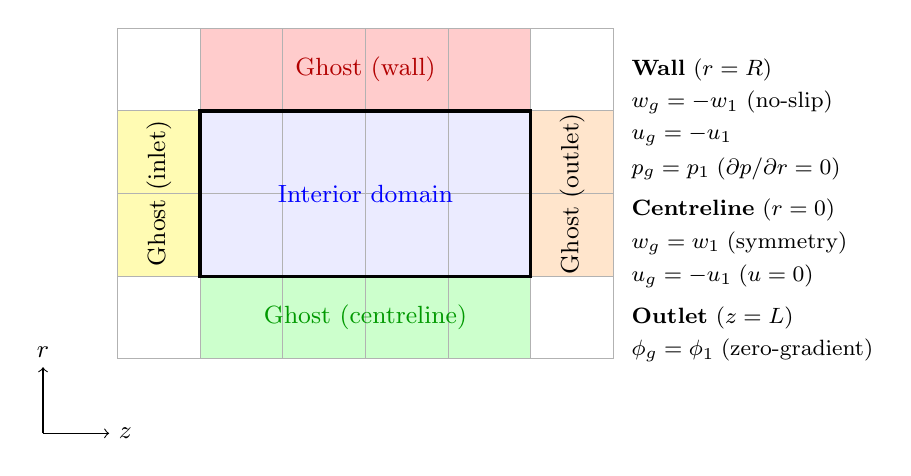
\begin{tikzpicture}[scale=1.05]
    % Physical domain
    \fill[blue!8] (1,1) rectangle (5,3);
    % Ghost: bottom (centreline r=0)
    \fill[green!20] (1,0) rectangle (5,1);
    % Ghost: top (wall r=R)
    \fill[red!20] (1,3) rectangle (5,4);
    % Ghost: left (inlet z=0)
    \fill[yellow!30] (0,1) rectangle (1,3);
    % Ghost: right (outlet z=L)
    \fill[orange!20] (5,1) rectangle (6,3);

    % Grid lines
    \draw[gray!60,thin] (0,0) grid (6,4);
    % Physical boundary
    \draw[black,very thick] (1,1) rectangle (5,3);

    % Arrows / axes -- kept in a clear corner, away from the ghost-band labels
    \draw[->] (-0.9,-0.9) -- (-0.9,-0.1) node[above,font=\small]{$r$};
    \draw[->] (-0.9,-0.9) -- (-0.1,-0.9) node[right,font=\small]{$z$};

    % Labels
    \node[blue,  font=\small] at (3,2)   {Interior domain};
    \node[green!60!black, font=\small] at (3,0.5)   {Ghost (centreline)};
    \node[red!70!black,   font=\small] at (3,3.5)   {Ghost (wall)};
    \node[font=\small, rotate=90] at (0.5,2)  {Ghost (inlet)};
    \node[font=\small, rotate=90] at (5.5,2) {Ghost (outlet)};

    % BC notes
    \node[font=\footnotesize, right] at (6.1,3.5) {\textbf{Wall} ($r=R$)};
    \node[font=\footnotesize, right] at (6.1,3.1) {$w_g = -w_1$ (no-slip)};
    \node[font=\footnotesize, right] at (6.1,2.7) {$u_g = -u_1$};
    \node[font=\footnotesize, right] at (6.1,2.3) {$p_g = p_1$\;($\partial p/\partial r=0$)};

    \node[font=\footnotesize, right] at (6.1,1.8) {\textbf{Centreline} ($r=0$)};
    \node[font=\footnotesize, right] at (6.1,1.4) {$w_g = w_1$\;(symmetry)};
    \node[font=\footnotesize, right] at (6.1,1.0) {$u_g = -u_1$\;($u=0$)};

    \node[font=\footnotesize, right] at (6.1,0.5) {\textbf{Outlet} ($z=L$)};
    \node[font=\footnotesize, right] at (6.1,0.1) {$\phi_g = \phi_1$\;(zero-gradient)};
\end{tikzpicture}
\caption{Ghost cell layout for the $(r,z)$ domain. Green: centreline symmetry; red: no-slip wall; yellow: inlet; orange: outlet. Subscript $g$ = ghost, subscript $1$ = first interior cell.}
\label{fig:cyl_uw_ghost}
\end{figure}

\begin{center}
\begin{tabular}{llll}
\toprule
Boundary & Condition & Variable & Ghost value \\
\midrule
Centreline ($r=0$) & $u=0$               & $u$ & $u_g = -u_1$ \\
                   & $\partial w/\partial r=0$ & $w$ & $w_g = w_1$ \\
                   & $\partial p/\partial r=0$ & $p$ & $p_g = p_1$ \\
\midrule
Wall ($r=R$)       & $u=0$, $w=0$        & $u$ & $u_g = -u_1$ \\
                   &                     & $w$ & $w_g = -w_1$ \\
                   & $\partial p/\partial r=0$ & $p$ & $p_g = p_1$ \\
                   & $\lambda\,\partial T/\partial r=q_w$ & $T$ & $T_g = T_1 + \frac{q_w\,\Delta r}{\lambda}$ \\
\midrule
Inlet ($z=0$)      & $u=0$, $w=W_\text{in}$ & $w$ & $w_g = 2W_\text{in}-w_1$ \\
                   &                        & $u$ & $u_g = -u_1$ \\
                   & $T=T_\text{in}$        & $T$ & $T_g = 2T_\text{in}-T_1$ \\
\midrule
Outlet ($z=L$)     & $\partial(\cdot)/\partial z=0$ & any & $\phi_g = \phi_1$ \\
\bottomrule
\end{tabular}
\end{center}
